\medskip

L'énoncé annonce des proportions, on va modéliser la situation de probabilité en assimilant les proportions à des probabilités.

\subsection*{Partie A}

\begin{enumerate}
	\item \begin{enumerate}
		\item D'après l'énoncé, on a donc :
	$P(V_1) = 1$ et, pour tout $n$ naturel supérieur ou égal à 2 : $P_{V_{n-1}}(V_n) = 0,9$ et aussi $P_{\overline{V_{n-1}}}\left(\overline{V_n}\right) = 0,9$. (une transmission fidèle, c'est quand les machines $n-1$ et $n$ détiennent la même valeur).

		On obtient l'arbre ci-contre :
		\hfill
		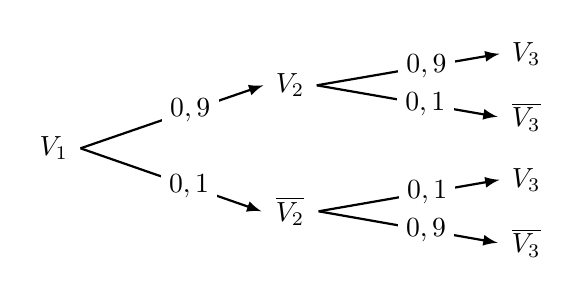
\begin{tikzpicture}[xscale=1,yscale=1,baseline={(R.base)}]
			
			\tikzstyle{fleche}=[->,>=latex,thick]
			\tikzstyle{noeud}=[fill=white,circle,inner sep=2pt]
			\tikzstyle{feuille}=[fill=white,circle,inner sep=2pt]
			\tikzstyle{etiquette}=[pos=0.6,fill=white, inner xsep=3pt, inner ysep=1.5pt]
			
			\def\DistanceInterNiveaux{3}
			\def\DistanceInterFeuilles{0.8}
			
			\def\NiveauA{(0)*\DistanceInterNiveaux}
			\def\NiveauB{(1)*\DistanceInterNiveaux}
			\def\NiveauC{(2)*\DistanceInterNiveaux}
			\def\InterFeuilles{(-1)*\DistanceInterFeuilles}
			
			\node[noeud] (R) at ({\NiveauA},{(1.5)*\InterFeuilles}) {$V_1$};
			\node[noeud] (Ra) at ({\NiveauB},{(0.5)*\InterFeuilles}) {$V_2$};
			\node[feuille] (Raa) at ({\NiveauC},{(0)*\InterFeuilles}) {$V_3$};
			\node[feuille] (Rab) at ({\NiveauC},{(1)*\InterFeuilles}) {$\overline{V_3}$};
			\node[noeud] (Rb) at ({\NiveauB},{(2.5)*\InterFeuilles}) {$\overline{V_2}$};
			\node[feuille] (Rba) at ({\NiveauC},{(2)*\InterFeuilles}) {$V_3$};
			\node[feuille] (Rbb) at ({\NiveauC},{(3)*\InterFeuilles}) {$\overline{V_3}$};
			
			\draw[fleche] (R.east)--(Ra.west) node[etiquette] {$0,9$};
			\draw[fleche] (Ra.east)--(Raa.west) node[etiquette] {$0,9$};
			\draw[fleche] (Ra.east)--(Rab.west) node[etiquette] {$0,1$};
			\draw[fleche] (R.east)--(Rb.west) node[etiquette] {$0,1$};
			\draw[fleche] (Rb.east)--(Rba.west) node[etiquette] {$0,1$};
			\draw[fleche] (Rb.east)--(Rbb.west) node[etiquette] {$0,9$};
		\end{tikzpicture}
		\hfill~

		\item Les évènements $V_2$ et $\overline{V_2}$ partitionnent l'univers, donc, d'après la loi des probabilités totales :

$P(V_3) = P\big(V_3 \cap V_2\big) + P\left(V_3 \cap \overline{V_2}\right) = 0,9 \times 0,9 + 0,1 \times 0,1 = 0,81 + 0,01 = 0,82$.

		On arrive bien à $P(V_3) = 0,82$.

		\item On demande de calculer : $P_{V_3}(V_2)$.

		D'après la définition, on a :\quad $P_{V_3}(V_2) = \dfrac{P(V_3 \cap V_2)}{P(V_3)} = \dfrac{0,9 \times 0,9}{0,82} = \dfrac{81}{82} \approx 0,988$.

		À $10^{-3}$ près, la probabilité que la machine 2 détienne 1, sachant que la machine 3 détient 1 est d'environ 0,988.
	\end{enumerate}

	\item \begin{enumerate}
		\item Soit $n$ un entier naturel non nul.

		Les évènements $V_n$ et $\overline{V_n}$ forment une partition de l'univers, donc, d'après la loi des probabilités totales :

		$\begin{aligned}
			p_{n+1} &= P(V_{n+1}) \\
			&= P\big(V_{n+1} \cap V_n\big) + P\big(V_{n+1} \cap \overline{V_n}\big)\\
			&= P_{V_n}\big(V_{n+1}\big)\times P\big(V_n\big) + P_{\overline{V_n}}\big(V_{n+1}\big)\times P\big(\overline{V_n}\big)\\
			&= 0,9\times P\big(V_n\big) + 0,1 \times  P\big(\overline{V_n}\big)\\
			&= 0,9\times p_n + 0,1 \times  (1 - p_n)\\
			&= 0,9p_n + 0,1 - 0,1 p_n\\
			&= 0,8 p_n + 0,1
		\end{aligned}$

		On arrive donc bien à la relation de récurrence annoncée pour la suite $(p_n)$.

		\item Pour tout entier naturel non nul $n$, on pose :

$P_n$ est l'affirmation :\quad \og $p_n = 0,5\times 0,8^{n-1} + 0,5$ \fg{}.

\textbf{Initialisation :} on a, d'après l'énoncé : \quad $p_1 = 1$,

et, par ailleurs, on a :\quad $0,5 \times 0,8^{1 - 1} + 0,5 = 0,5 + 0,5 = 1$.

On constate donc que l'affirmation $P_1$ est vraie.

\textbf{Hérédité :} soit $n$ naturel non nul donné tel que l'affirmation $P_n$ est vraie.

D'après l'hypothèse de récurrence :

$\begin{aligned}
p_n = 0,5 \times 0,8^{n-1} + 0,5
	&\implies 0,8p_n = 0,8\left(0,5 \times 0,8^{n-1} + 0,5\right) \\
	&\implies 0,8p_n = 0,5 \times 0,8^{n-1} \times 0,8 + 0,4 \\
	&\implies 0,8p_n = 0,5 \times 0,8^{n} + 0,4 \\
	&\implies 0,8p_n + 0,1 = 0,5 \times 0,8^{n} + 0,4 + 0,1\\
	&\implies 0,8p_n + 0,1 = 0,5 \times 0,8^{n} + 0,5\\
	&\implies p_{n+1} = 0,5 \times 0,8^{n} + 0,5\quad \text{c'est }P_{n+1}\\
\end{aligned}$

\textbf{Conclusion :} on a prouvé que l'affirmation $P_1$ est vraie, et que, $n$ étant un naturel non nul, la véracité de $P_n$ entraîne celle de $P_{n+1}$. En vertu du principe de récurrence, on peut conclure que :

$\forall n \in \N^{*},\quad u_n = 0,5 \times 0,8^{n-1} + 0,5$.

Autrement dit, on a établi par récurrence une expression explicite du terme général $p_n$.

		\item Pour tout $n$ entier naturel non nul, on a : \quad $\begin{aligned}[t]
			0,5 \times 0,8^{n-1} &= \dfrac{0,5}{0,8} \times 0,8^{n} \\&= 0,625 \times 0,8^n.
		\end{aligned}$

		Comme on a :\quad $-1 < 0,8 < 1$\quad la propriété des limites de suites géométriques donne : \quad $\lim\limits_{n \to +\infty} 0,8^n = 0$, puis $\lim\limits_{n \to +\infty} 0,625 \times 0,8^n = 0$.

Puis, par limite de la somme, on a :\quad $\lim\limits_{n \to +\infty} p_n = \lim\limits_{n \to +\infty} 0,625 \times 0,8^n + 0,5 = 0,5$.

Ainsi, quand le nombre de machines tend vers plus l'infini, la probabilité que la dernière machine détienne la valeur 1 tend vers 0,5.
	\end{enumerate}
\end{enumerate}

\subsection*{Partie B}

\begin{enumerate}
	\item L'instruction de la ligne 5 est une instruction conditionnelle : elle indique l'instruction de la ligne suivante ne s'exécutera qu'à la condition que le test \texttt{rand() < 0.1} renvoie la valeur \texttt{True}.

Or, l'instruction \texttt{rand()} renvoie un nombre aléatoire dans $[0~;~1[$, donc la probabilité que ce nombre soit strictement inférieur à 0,1, c'est-à-dire dans l'intervalle $[0~;~0,1[$ est proportionnelle à l'amplitude de cet intervalle, la probabilité que cela arrive est donc de $\dfrac{0,1 - 0}{1 - 0} = 0,1$.

\emph{La ligne 5 va rendre l'exécution de la ligne 6 aléatoire, avec une probabilité que la ligne 6 s'exécute égale à 0,1.}

C'est-à-dire que la ligne 6 doit avoir pour effet de "mal transmettre" la dernière donnée détenue, qui est stockée dans la variable \texttt{donnee}. Cette variable contient 0 ou 1. Si elle contenait 0, après la ligne 6 elle contiendra $1 - 0 = 1$, soit la valeur contraire. Si elle contenait 1, après la ligne 6, elle contiendra $1 - 1 = 0$, là encore, la valeur contraire.

\emph{La ligne 6 a donc pour effet de modifier la donnée, pour simuler une transmission contraire.}

	\item Si l'appel \texttt{simulation(4)} renvoie \texttt{[1,1,1,1,1]}, cela signifie que l'on a eu 4 transmissions fidèles, entre 5 machines.

La probabilité que cela arrive est donc  :

$0,9 \times 0,9 \times 0,9 \times 0,9 = 0,9^{4} = \np{0,6561}\approx 0,656$.

De façon analogue l'appel \texttt{simulation(6)} renvoie une simulation de 6 transmissions entre 7 machines.

Si l'appel renvoie \texttt{[1,0,1,0,0,1,1]}, cela signifie que les trois premières transmissions sont contraires (de 1 à 0, puis de 0 à 1, puis de 1 à 0), la quatrième transmission est fidèle (de 0 à 0), la cinquième est contraire (de 0 à 1) et la sixième et dernière est fidèle (de 1 à 1).

La probabilité que cela arrive est donc  :

$0,1 \times 0,1 \times 0,1 \times 0,9 \times 0,1 \times 0,9 = 0,9^{2}\times 0,1^{4} = 8,1\times 10^{-5}\approx 0,000$.

À $10^{-3}$ près, la probabilité d'obtenir \texttt{[1,1,1,1,1]} est d'environ 0,656, celle d'obtenir \texttt{[1,0,1,0,0,1,1]} est d'environ 0,000.
\end{enumerate}
